\documentclass[12pt, a4 paper]{article}
\usepackage{geometry}
\geometry{left=2cm, right=2cm, top=1.5cm, bottom=1.5cm}
\usepackage{amsmath}
\usepackage{amssymb}
\usepackage{amsfonts}
\usepackage{framed}
\usepackage{caption}
\usepackage{indentfirst}
\usepackage{graphicx}
\usepackage{pythonhighlight}

\begin{document}

    %%%%%%%%%%%%%%%%%%%%%%%%%%%%%%%%%%%%%%   Q1   %%%%%%%%%%%%%%%%%%%%%%%%%%%%%%%%%%%%%%%%%
    \begin{framed}
        \section{[Q1]}
        Last week, we talked about Lagrange.
    \end{framed}

    %%%%%%%%%%%%%%%%%%%%%%%%%%%%%%%%%%%%%%   Q2   %%%%%%%%%%%%%%%%%%%%%%%%%%%%%%%%%%%%%%%%%
    \begin{framed}
        \section{[Q2]}
        done
    \end{framed}

    \begin{framed}
        \section{[Q3]}
        \subsection{(a)}
        \begin{equation}
            \lVert x \rVert_{\infty} = \max{\{ \lvert x \rvert \}}
            = \left\{
                \begin{array}{lcl}
                x      & {x      \geq      0}\\
                -x     & {x      <      0}\\
                \end{array} \right. 
        \end{equation}
        \indent Hence, the gradient of $\lVert x \rVert_{\infty}$ is,
        \begin{equation}
            \partial \lVert x \rVert_{\infty} 
            = \left\{\begin{array}{lcl}
                1      & {x      \geq      0}\\
                -1     & {x      <      0}\\
            \end{array} \right. 
        \end{equation}
        \indent And we can write it as,
        \begin{equation}
            \partial \lVert x \rVert_{\infty} = \left\{
                u: \lVert u \rVert_{1}=1, u^{T}x = 
                \lVert x \rVert_{\infty}
            \right\}
        \end{equation}

        \subsection{(b)}
        
    \end{framed}

\begin{framed}
    \section{[Q7]}
    \subsection{(a)}
    According to KKT condtion (K1), we have,
    \begin{equation}
        (x-2)(x-4) \leq 0
    \end{equation}
    \indent the feasible set is $ \left\{x: 2 \leq x \leq 4 \right\} $

    \subsection{(b)}
    The Lagrangian for this problem is,
    $$
        L(x, \lambda) = x^{2}+1 + \lambda (x-2)(x-4)
    $$
    \indent According to KKT conditions (K4), we have,
    $$
    \frac{\partial{L}}{\partial x} = 2x + 2\lambda x - 6\lambda
    $$
    \indent Set it to 0, we can get $x$ as follows,
    $$
    x = \frac{3\lambda}{\lambda + 1}
    $$
    \indent Lagrange dual program is
    $$
    \mathop{\text{maximize}}_{\lambda} \frac{-\lambda^{3} +
    8\lambda^{2} + 10\lambda + 1}{(\lambda+1)^{2}}, \quad
    \text{subject to } \lambda \geq 0
    $$
    \indent Apprently, this will be maximize when $\lambda=2$,
    which, when substituted into the dual problem yields,
    $$
    d(\lambda^{\star}) = 5
    $$
    \indent Hence, the optimal $x^{\star}$ is \textbf{2}, accordingly,
    the value of the objective function at the minimizer is \textbf{5}.

    \subsection{(c)}
    {\centering
    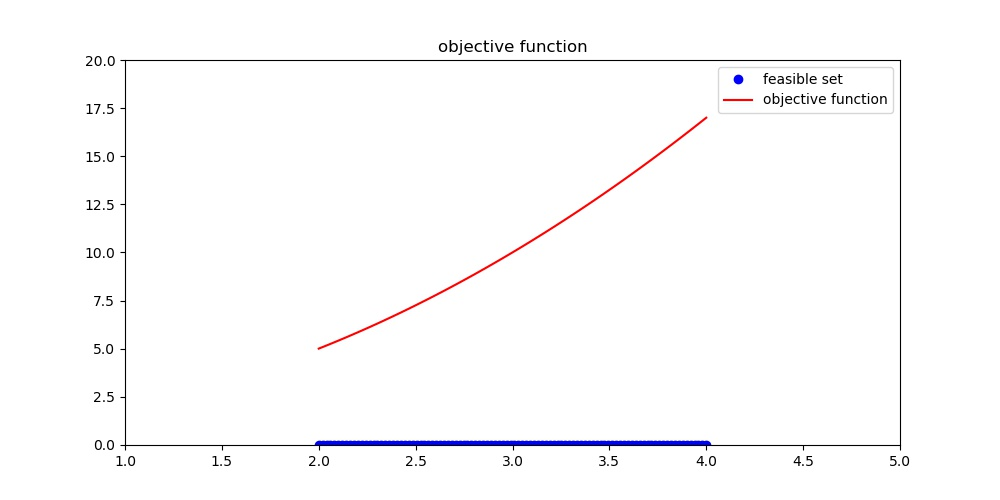
\includegraphics[width=10cm, height=5cm]{7c.jpg}
    \captionof{figure}{Plot of Objective Function} 
    }
    {\centering
    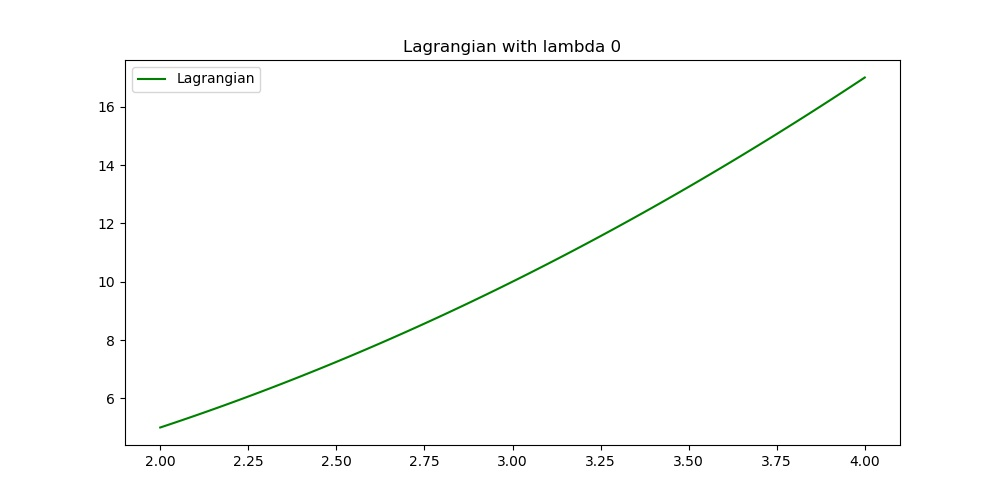
\includegraphics[width=10cm, height=5cm]{7c-lam0.jpg}
    \captionof{figure}{Plot of Lagrangian with $\lambda=0$} 
    }
    {\centering
    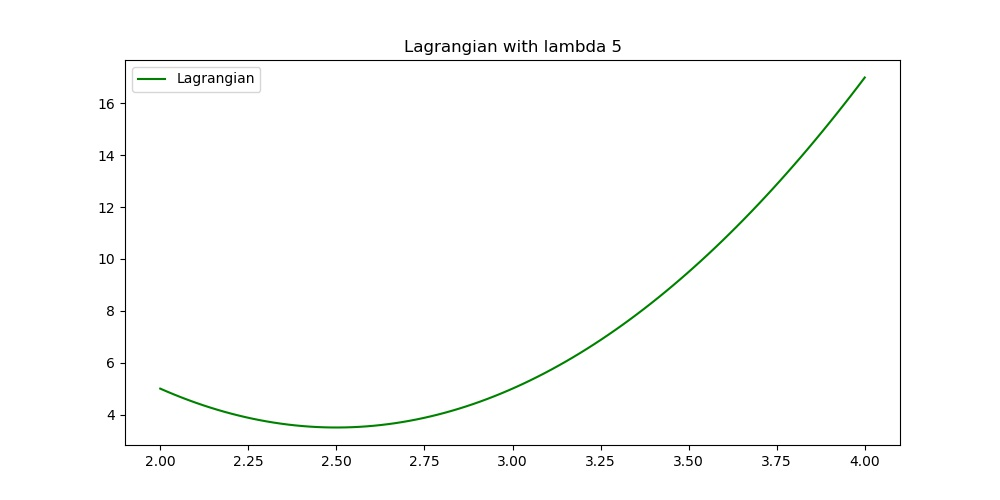
\includegraphics[width=10cm, height=5cm]{7c-lam5.jpg}
    \captionof{figure}{Plot of Lagrangian with $\lambda=5$} 
    }
    {\centering
    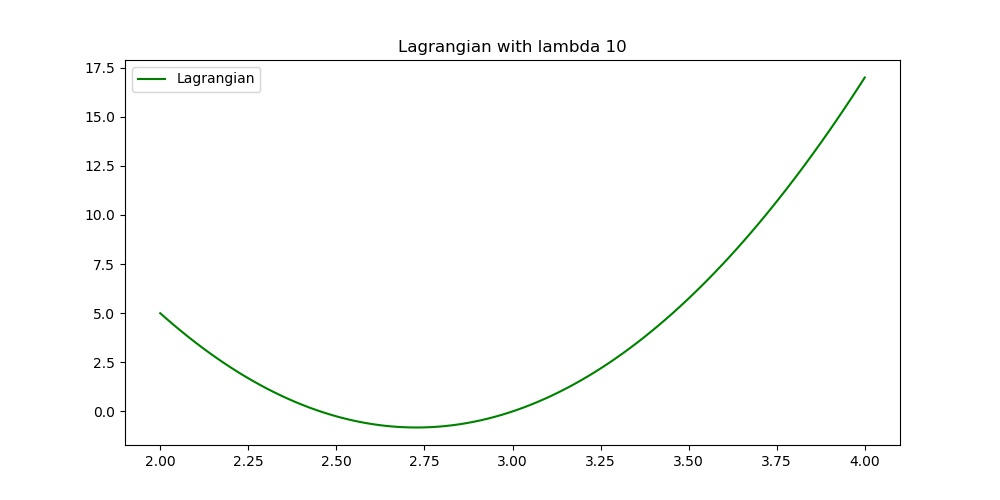
\includegraphics[width=10cm, height=5cm]{7c-lam10.jpg}
    \captionof{figure}{Plot of Lagrangian with $\lambda=10$} 
    }

    \subsection{(d)}
    {\centering
    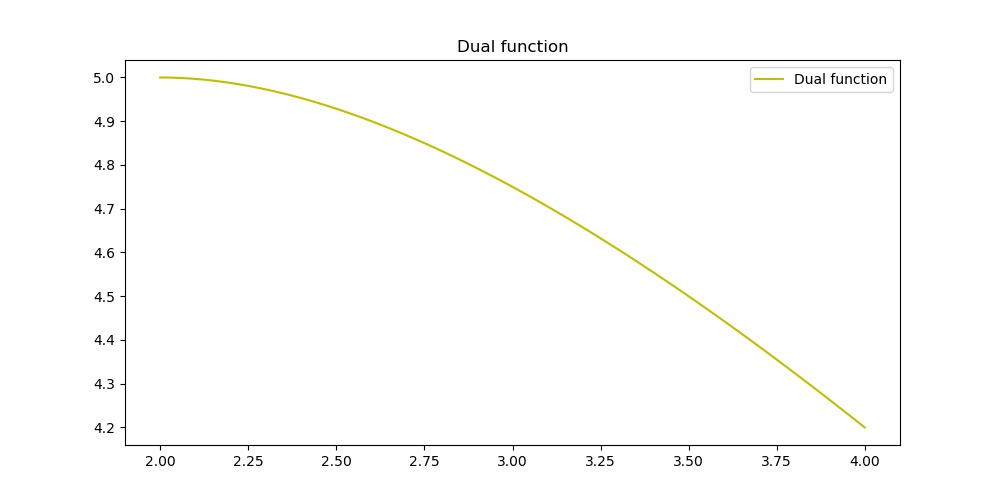
\includegraphics[width=10cm, height=5cm]{7d.jpg}
    \captionof{figure}{Plot of Dual function} 
    }

    \subsection{(e)}
    The dual problem is
    $$
    \mathop{\text{maximize}}_{\lambda} \frac{-\lambda^{3} +
    8\lambda^{2} + 10\lambda + 1}{(\lambda+1)^{2}}, \quad
    \text{subject to } \lambda \geq 0
    $$
    \indent And the maximizer $\lambda^{\star} = 2$, accordingly
    $d(\lambda^{\star}) = 5$.\\
    \indent Strong duality holds because the value of primal problem
    $p^{\star}$ is \textbf{5} and the value of dual problem $d^{\star}$
    is \textbf{5}.
\end{framed}



\end{document}